\documentclass[a4paper]{article}
\usepackage[affil-it]{authblk}
\usepackage{float}
\usepackage{amsmath, amssymb, amsthm, amsfonts}
% \usepackage[backend=bibtex,style=numeric]{biblatex}
\usepackage{graphicx}

\usepackage{hyperref}
% 设置超链接样式
\hypersetup{
	colorlinks=true,
	linkcolor=blue,
	citecolor=blue,
	urlcolor=blue,
}

\usepackage{geometry}
\geometry{margin=1.5cm, vmargin={0pt,1cm}}
\setlength{\topmargin}{-1cm}
\setlength{\paperheight}{29.7cm}
\setlength{\textheight}{25.3cm}

% \addbibresource{citation.bib}

\begin{document}
% =================================================
\title{Numerical Analysis homework \# 2}

\author{Wanghao 3220104819
  \thanks{Electronic address: \texttt{3220104819@zju.edu.cn}}}
\affil{(Mathematics and Applied Mathematics 2201), Zhejiang University }


\date{Due time: \today}

\maketitle

% \begin{abstract}
%     The abstract is not necessary for the theoretical homework, 
%     but for the programming project, 
%     you are encouraged to write one.      
% \end{abstract}


% ============================================
\section*{I. Error and Its Bounds About Interpolation}

\subsection*{I-a Find $\xi(x)$}

For $f(x) = \frac{1}{x}, x_0=1, x_1=2$, we can easily get the Interpolation polynomial $p_1(f; x)$ as follows:

\begin{equation}
  p_1(f; x) = f(x_0) \frac{x-x_1}{x_0-x_1} + f(x_1) \frac{x-x_0}{x_1-x_0} = -\frac{1}{2} x + \frac{3}{2} 
\end{equation}

So by $f(x) - p_1(f; x) = \frac{f^{\prime \prime} (\xi (x))}{2} (x-x_0) (x-x_1)$, we can get $\xi(x)$ as follows:

\begin{equation}
  \begin{aligned}
    f^{\prime \prime} (\xi (x)) &= \frac{2}{x} \\
    \Rightarrow \xi (x) = &\sqrt[3]{x}
  \end{aligned}
\end{equation}

\subsection*{I-b Find the Bounds of $\xi(x)$}

We already know that $\xi(x) = \sqrt[3]{x}$, so in the domain $[1,2]$, we can easily know that:

\begin{equation}
  \min \xi(x) = \sqrt[3]{1} = 1, \quad \max \xi(x) = \sqrt[3]{2}
\end{equation}

$f^{\prime \prime}(\xi(x)) = \frac{2}{x}$. Therefore we can know that:

\begin{equation}
  \max f^{\prime \prime}(\xi(x)) = \frac{2}{1} = 2
\end{equation}

\section*{II. Interpolation on $\mathbb{P}_{m}^+$}

In order to find $p \in \mathbb{P}_{2n}^+ = \{p: p\in \mathbb{P}_{2n}, \forall x\in\mathbb{R}, p(x)\ge 0\}$, we need to find new basis functions $\{l_i(x)\}_{i=0}^{n}$, which $l_i \in \mathbb{P}_{2x}^+$. 

It is easy to know that the following functions are enough:

\begin{equation}
  l_i(x) = \prod_{k=0, k\neq i}^{n} \cfrac{(x-x_k)^2}{(x_i-x_k)^2}, \quad i=0,1,\cdots,n
\end{equation}

which satifies $l_i(x_i) = 1, l_i(x_j) = 0, j\neq i, l_i(x) \ge 0, \forall x\in\mathbb{R}$.

So the polynomial $p \in \mathbb{P}_{2n}^+$ such that $p(x_i) = f(x_i) \ge 0, i=0,1,\cdots,n$ can be written as follows:

\begin{equation}
  p(x) = \sum_{i=0}^{n} f(x_i) l_i(x) = \sum_{i=0}^{n} f(x_i) \prod_{k=0, k\neq i}^{n} \cfrac{(x-x_k)^2}{(x_i-x_k)^2}
\end{equation}

\section*{III. Evaluation for Exponential Function}

\subsection*{III-a. Calculate $f[t,t+1,\cdots, t+n]$}

In order to prove when $f(x) = e^t$ then $\forall t\in \mathbb{R}, f[t,t+1,\cdots, t+n] = \frac{(e-1)^n}{n!}e^t$

\begin{itemize}
  \item When $n=0$, we can easily know that $f[t] = e^t = \frac{(e-1)^0}{0!}e^t$
  \item Assume then when $n=k$, the equation holds, i.e. $f[t,t+1,\cdots, t+k] = \frac{(e-1)^k}{k!}e^t$
  
  Then, for $n=k+1$, we can easily know that:

  \begin{equation}
    \begin{aligned}
      f[t,t+1,\cdots, t+k+1] &= \frac{f[t+1,\cdots, t+k+1] - f[t,t+1,\cdots, t+k]}{(t+k+1) - t} \\
                             &= \frac{\frac{(e-1)^k}{k!} (e^{t+1} - e^t)}{k+1} \\
                             &= \frac{(e-1)^{k+1}}{(k+1)!}e^t
    \end{aligned}
    \label{eq::III-a.1}
  \end{equation}

  The equation holds for $n=k+1$.
\end{itemize}

Therefore, we can know that $\forall t\in \mathbb{R}, f[t,t+1,\cdots, t+n] = \frac{(e-1)^n}{n!}e^t$

\subsection*{III-b. Error Estimation}

From the equation \ref{eq::III-a.1}, we can know that:

\begin{equation}
    f[t,t+1,\cdots, t+n] = \frac{(e-1)^n}{n!}e^t, \forall t\in \mathbb{R}
\end{equation}

Therefore, we can easily know that:

\begin{equation}
  \begin{aligned}
    f[0,1,\cdots, n] &= \frac{(e-1)^n}{n!} = \frac{f^{(n)}(\xi)}{n!} = \frac{e^{\xi}}{n!} \\
    \Rightarrow \xi &= n \ln(e-1) \approx 0.5413n
  \end{aligned}
\end{equation}

Therefore, $\xi = n \ln(e-1)$, and $\xi$ is to the right of the midpoint $\frac{n}{2}$

\section*{IV. Application of Newton Interpolation}

\subsection*{IV-a. Find the Newton Interpolation Polynomial}

For $f(0)=5, f(1)=3, f(3)=5, f(4)=12$, we can know that $f[0]=5, f[1]=3, f[3]=5, f[4]=12$. Draw table like this:

\begin{table}[H]
  \centering
  \begin{tabular}{c|cccc}
    0 & 5  &    &   &\\
    1 & 3  & -2 &   &\\
    3 & 5  & 1  & 1 &\\
    4 & 12 & 7  & 2 & $\frac{1}{4}$\\
  \end{tabular}
  \label{tabel::IV-A.tabel1}
\end{table}

The above table \ref{tabel::IV-A.tabel1} is given by $f[x_0,x_1,\cdots,x_n] = \frac{f[x_1,\cdots,x_n] - f[x_0,x_1,\cdots,x_{n-1}]}{x_n - x_0}$ 

so we can know that $f[0]=5, f[0,1]=-2, f[0,1,3]=1, f[0,1,3,4]=\frac{1}{4}$

So the Newton Interpolation is:

\begin{equation}
  \begin{aligned}
    p_3(f;x) &= f[0] + f[0,1](x-0) + f[0,1,3](x-0)(x-1) + f[0,1,3,4](x-0)(x-1)(x-3) \\
             &= 5 - 2x + x(x-1) + \frac{1}{4}x(x-1)(x-3)
  \end{aligned}
\end{equation}

\section*{IV-b. Minimum value of $p_3(f;x)$}

In order to find the approximate minimum value of $f(x)$ in $x\in (1,3)$, we can just analyze the minimum value of $p_3(f;x) = p(x)$ in $x\in(1,3)$.

Its easy to show $p(x) = \frac{1}{4}x^3 - \frac{9}{4}x + 5$, so we can know that 

\begin{equation}
  p^{\prime}(x) = \frac{3}{4}x^2 - \frac{9}{4} = 0 \Rightarrow x = \sqrt{3}
\end{equation}

Therefore, the minimum value of $p(x)$ in $x\in(1,3)$ is $p(\sqrt{3}) = 5 - \frac{3}{2}\sqrt{3}$, $x_{\min} = \sqrt{3}$

\section*{V. The Generalized Newton Interpolation}

\subsection*{V-a. Compute the Generalized Newton Interpolation}

To compute $f[0,1,1,1,2,2]$, we can draw the table like this:

\begin{table}[H]
  \centering
  \begin{tabular}{c|cccccc}
    0 & $f[0]$ &                 &                                  & & & \\
    1 & $f[1]$ & $f[0,1]$        &                                  & & & \\
    1 & $f[1]$ & $f^{\prime}(1)$ & $f[0,1,1]$                       & & & \\
    1 & $f[1]$ & $f^{\prime}(1)$ & $\frac{f^{\prime \prime}(1)}{2}$ & $f[0,1,1,1]$ & & \\
    2 & $f[2]$ & $f[1,2]$        & $f[1,1,2]$                       & $f[1,1,1,2]$ & $f[0,1,1,1,2]$ & \\
    2 & $f[2]$ & $f^{\prime}(2)$ & $f[1,2,2]$                       & $f[1,1,2,2]$ & $f[1,1,1,2,2]$ & $f[0,1,1,1,2,2]$ \\
  \end{tabular}
  \label{tabel::V-A.tabel1}
\end{table}

We can know that $f(x) = x^7, f^\prime(x)=7x^6, f^{\prime \prime}(x) = 42x^5$, so put them into the table \ref{tabel::V-A.tabel1}, we can get:

\begin{table}[H]
  \centering
  \begin{tabular}{c|cccccc}
    0 & 0   &     &     &     &     & \\
    1 & 1   & 1   &     &     &     & \\
    1 & 1   & 7   & 6   &     &     & \\
    1 & 1   & 7   & 21  & 15  &     & \\
    2 & 128 & 127 & 120 & 99  & 42  & \\
    2 & 128 & 448 & 321 & 201 & 102 & 30 \\
  \end{tabular}
  \label{tabel::V-A.tabel2}
\end{table}

So $f[0,1,1,1,2,2] = 30$

\subsection*{V-b. Determin $\xi$}
We know that $f[0,1,1,1,2,2] = \frac{f^{(5)}(\xi)}{5!}$, and $f^{(5)}(x) = 2520x^2$, so we can know that:

\begin{equation}
  \begin{aligned}
    30 &= f[0,1,1,1,2,2] = \frac{f^{(5)}(\xi)}{5!} = \frac{2520\xi^2}{5!} \\
    \Rightarrow \xi &= \sqrt{\frac{5! \times 30}{2520}} = \sqrt{\frac{10}{7}} \approx 1.1952
  \end{aligned}
\end{equation}

\section*{VI. }

% ===============================================
\section*{ \center{\normalsize {Acknowledgement}} }
% The section title is generated by \textbf{Kimi}, with a little revise. 
% \begin{figure}[H]
%   \begin{center}
%     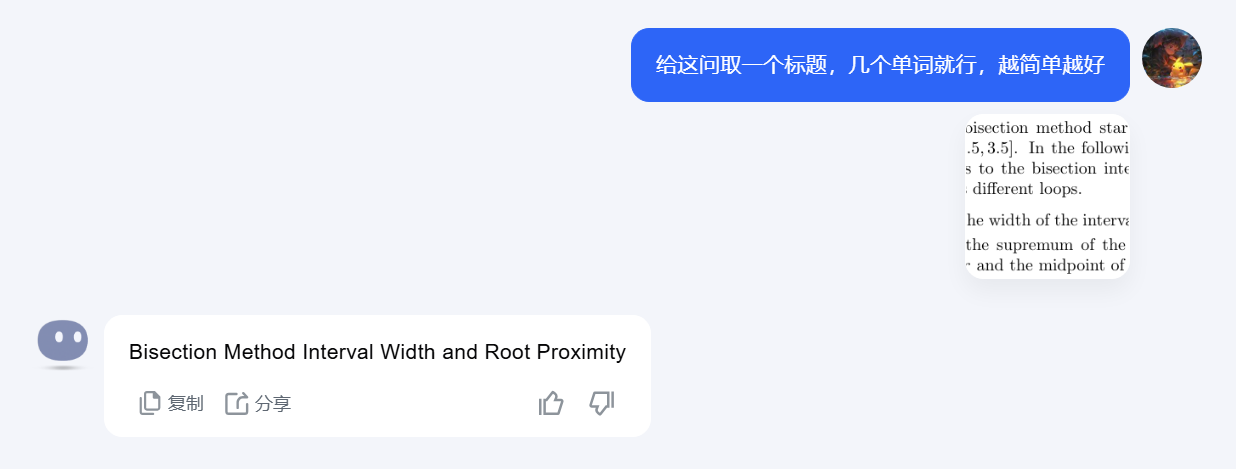
\includegraphics[width=0.8\textwidth]{./figure/kimi.png}
%   \end{center}
% \end{figure}

% \printbibliography


\end{document}